\subsection*{1.1 Ladung Q [C]}

\begin{itemize}
    \item Elementarladung: $q_{Elektron} = e = - 1.602 \cdot 10^{-19}C$
\end{itemize}

Coulomb-Kraft: \mathbox{\overrightarrow{F_C}=\frac{1}{4\pi\varepsilon_0}\cdot \frac{q_1 \cdot q_2}
{r^2}\cdot \overrightarrow{e_r}}

\begin{itemize}
    \item Ladungen mit gleichem Vorzeichen stossen sich ab.
    \\$F_C<0 \rightarrow \text{abstossend}$,
    $F_C>0 \rightarrow \text{anziehend}$
    \item Ladungen leitender Körper stets an Oberfläche.\\
    $\rightarrow$ Inneres: Ladungs und Feldfrei
\end{itemize}

\subsubsection*{Ladungsdichte}

\begin{itemize}
    \item Liniendichte $\lambda$: \mathbox{\lambda = \frac{Q}{l} \left[\frac{C}{m}\right]}
    \item Oberflächendichte $\sigma$: \mathbox{\sigma = \frac{Q}{A} \left[\frac{C}{m^2}\right]}
    \item Volumendichte $\rho$: \mathbox{\rho = \frac{Q}{l} \left[\frac{C}{m^3}\right]}
\end{itemize}


%Stromstärke: \mathbox{I = \frac{dQ}{dt}}
%Ladung: \mathbox{Q = \int\limits_{\Delta t} I dt}
%Widerstand: \mathbox{R = \frac{U}{I}, I \sim U}

%\begin{tabular}{c c}
%    Ohmsche Leiter & nicht-ohmsche Leiter \\
%    $I = \frac{U}{R}$ & $R_{\text{diff}} = \frac{dU}{dI}$\\
%    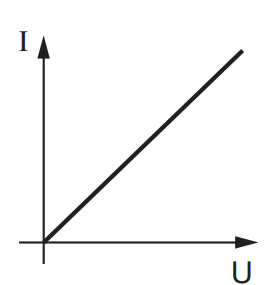
\includegraphics[width = 30mm]{src/images/plot_ohmscher_leiter.png} & 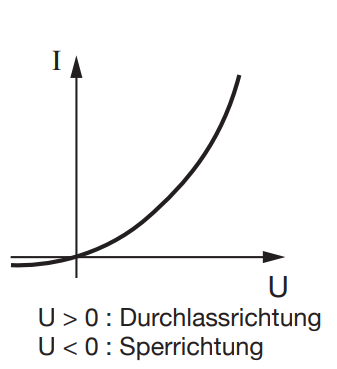
\includegraphics[width = 30mm]{src/images/plot_nicht-ohmscher_leiter.png}
%\end{tabular}

